%!TEX TS-program = xelatex

% -- Document Class -----------------------------------------------------------

\documentclass[a4paper, 12pt]{article}

% -- Imports ------------------------------------------------------------------

% Common packages
% -- Common Packages ----------------------------------------------------------

% Language
\usepackage{polyglossia}
    \setmainlanguage{english}
    \setotherlanguage{german}
% Context sensitive quotation
\usepackage{csquotes}
% Citations
\usepackage[style=alphabetic, backend=biber]{biblatex}
\IfFileExists{References.bib}{\addbibresource{References.bib}}{}
% Support highlighting of certain parts of the text
\usepackage{framed}
% Support for unicode math fonts
\usepackage{unicode-math}
% Extended color support
\usepackage[x11names]{xcolor}

% Document specific packages
% -- Document Packages --------------------------------------------------------

% Customize enumerations
\usepackage{enumitem}
% Extend options for positioning floats
\usepackage{float}
% Support spaces in filenames
\usepackage{grffile}
% Headers & Footers
\usepackage[automark, nouppercase]{scrpage2}
% Emphasize text
\usepackage{soul}
% Support for changing the format of titles
\usepackage{titlesec}
% Extras for XƎTEX
\usepackage{xltxtra}
% Hyperlinks and PDF properties
\usepackage{hyperref}

% Document specific properties
% -- Includes -----------------------------------------------------------------

% Document Attributes
% -- Document Attributes ------------------------------------------------------

\newcommand{\Title}{Exercises}
\newcommand{\TitleDescription}{Computer Aided Verification}
\newcommand{\Version}{1}
\newcommand{\Subject}{Solutions for the exercises of the course Computer Aided
                      Verification}
\newcommand{\KeyWords}{LTL, CTL, Temporary Logic}
\newcommand{\LeftFooter}{\Title~—~\TitleDescription}

\newcommand{\AuthorOne}{René Schwaiger}
\newcommand{\MailOne}{\href{mailto:sanssecours@f-m.fm}{sanssecours@f-m.fm}}

% Color Definitions And Syntax Highlighting
% -- Color definitions --------------------------------------------------------

\definecolor{aqua}{rgb}         {0,     0.56,   1}
\definecolor{bluegray}{rgb}     {0.22,  0.46,   0.84}
\definecolor{grape}{rgb}        {0.56,  0,      1}
\definecolor{lightgray}{rgb}    {0.94,  0.94,   0.94}
\definecolor{orchid}{rgb}       {0.41,  0.13,   0.55}
\definecolor{orange}{rgb}       {1,     0.54,   0}
\definecolor{silver}{rgb}       {0.57,  0.57,   0.57}
\definecolor{turquoise}{rgb}    {0,     0.86,   0.84}

% -- Syntax Highlighting ------------------------------------------------------

% Background color for syntax highlighting
\definecolor{bgcolor}{rgb}      {1,     1,      1}

% Syntax highlighting definitions
% Text
\newcommand{\hlstd}[1]{\textcolor{black}{#1}}
% Numbers
\newcommand{\hlnum}[1]{\textcolor{DarkOrchid4}{#1}}
\newcommand{\hlesc}[1]{\textcolor[rgb]{1,0,1}{#1}}
% Strings
\newcommand{\hlstr}[1]{\textcolor{SeaGreen3}{#1}}
\newcommand{\hlpps}[1]{\textcolor[rgb]{0.51,0.51,0}{#1}}
% Comments
\newcommand{\hlslc}[1]{\textcolor{aqua}{#1}}
\newcommand{\hlcom}[1]{\textcolor{aqua}{#1}}
\newcommand{\hlppc}[1]{\textcolor[rgb]{0,0.51,0}{#1}}
\newcommand{\hlopt}[1]{\textcolor[rgb]{0,0,0}{#1}}
\newcommand{\hllin}[1]{\textcolor[rgb]{0.33,0.33,0.33}{#1}}
% Keywords
\newcommand{\hlkwa}[1]{\textcolor{DodgerBlue3}{#1}}
\newcommand{\hlkwb}[1]{\textcolor[rgb]{0,0.34,0.68}{#1}}
\newcommand{\hlkwc}[1]{\textcolor{DarkOrchid4}{#1}}
% Functions
\newcommand{\hlkwd}[1]{\textcolor{orange}{#1}}

% Fonts
% -- Font Properties ----------------------------------------------------------

% Use same size for numbers and other text
\defaultfontfeatures{Numbers=Lining}

% Set fonts for document
\setmainfont[Mapping=tex-text]{Avenir Next}
\setsansfont[Mapping=tex-text]{Ubuntu}
\setmonofont[Scale=MatchLowercase]{Menlo}
\setmathfont{Asana-Math.otf}
\setmathfont[range=\mathtt, Scale=MatchLowercase]{Menlo}

% Define font styles
\newfontfamily\Zapfino{Zapfino}

% Headers And Footers
% -- Headers And Footers ------------------------------------------------------

% Use normal font instead of italic font for head
\renewcommand{\headfont}{\normalfont}

% Set headers and footers
\ihead{\headmark}
\ohead{}
\ifoot{\LeftFooter}
\ofoot{\thepage}

% Set height of head
\setlength{\headheight}{1.8\baselineskip}

% Set thickness of separation line in header, footer
\setheadsepline{0.5pt}
\setfootsepline{0.5pt}


% -- Hyperref properties ------------------------------------------------------

\hypersetup
{
    pdftitle    = {\Title},
    pdfsubject  = {\Subject},
    pdfauthor   = {\AuthorOne},
    pdfkeywords = {\KeyWords},
    colorlinks  = true,
    linkcolor   = black,
    anchorcolor = black,
    citecolor   = silver,
    urlcolor    = orange
}

% -- Other --------------------------------------------------------------------

% No indentation after paragraphs
\setlength\parindent{0cm}
% Background color for highlighted text
\sethlcolor{lightgray}

% Custom macros
% -- Macros -------------------------------------------------------------------

\newcommand{\codeinput}[1]
{
    \begin{leftbar}
        \input{Code/#1}
    \end{leftbar}
}

\newcommand{\code}[1]
{
    \hl{\texttt{#1}}
}


% -- Document -----------------------------------------------------------------

\begin{document}
% -- Title-Page ---------------------------------------------------------------

\begin{titlepage}
    \begin{center}
        % Title and title-description
        {\Huge\Zapfino\Title}
        \vskip 0.5cm
        {\color{aqua}\hrule}
        \vskip 0.5cm
        {\Large\textit\TitleDescription}
        \vskip 14cm
    \end{center}

    % Document information
    \begin{leftbar}
        \begin{tabular}{ll}
            \textbf{Author}  & \AuthorOne\\
            \textbf{Mail}    & \MailOne\\
            \textbf{Version} & \Version\\
            \textbf{Date}    & \today
        \end{tabular}
    \end{leftbar}

\end{titlepage}

% -- Table of Contents --------------------------------------------------------

% Set section format for table of contents
\titleformat{\section}{\sffamily\bfseries}{}{0pt}{}[{\color{aqua}\hrule}]

% Set separation of dots between name of section and page number to such a high
% value that there will be no points in the table of contents
\makeatletter \renewcommand{\@dotsep}{10000} \makeatother
% Use blank header and footer
\pagestyle{empty}
% Start on new page
\newpage
% The table of contents starts at the second page
\setcounter{page}{2}
% Set table of contents
\tableofcontents

% -- Section & Paragraph Style ------------------------------------------------

% Set format for section
\titleformat{\section}
    {\large\sffamily\bfseries}  % Large, bold, sans serif font for section
    {}                          % No format applied to whole title
    {0pt}                       % No separation between label and title
    {\thesection~·~}            % Start with section number
    [{\color{aqua}\hrule}]      % Underline with blue ruler

% Set format for other sections and paragraphs
% Color = orchid, Font = bold, sans serif
\titleformat*{\subsection}{\color{orchid}\sffamily\bfseries}
\titleformat*{\subsubsection}{\color{orchid}\sffamily\bfseries}
\titleformat*{\paragraph}{\color{orchid}\sffamily\bfseries}
\titleformat*{\subparagraph}{\color{orchid}\sffamily\bfseries}

% -- Page Style ---------------------------------------------------------------

% Start with text on a new page
\newpage
% Display headers and footers
\pagestyle{scrheadings}


% -- Text ---------------------------------------------------------------------

\section{Exercise 1}

\newcommand{\LFP}{\mathbf{lfp}~Z~[τ(Z)]}
\newcommand{\GFP}{\mathbf{gfp}~Z~[τ(Z)]}

Show the results about $\mathbf{lfp}$ on slides 4 and 5 of “alecture3.pdf”.

\paragraph{Slide 4}

Let $τ: Pred(S) → Pred(S)$ be a predicate transformer, then:

\begin{enumerate}

    \item If $τ$ is monotonic then it has a least fixed-point $\LFP$, and a greatest fixed-point $\GFP$.

    \item $\LFP = ∩\{ Z ∣ τ(Z) = Z \}$ whenever $τ$ is monotonic.

    \item $\LFP = ∪ᵢτⁱ(False)$ whenever $τ$ is also $∪$-continuous;

    \item $\GFP = ∪\{ Z ∣ τ(Z) = Z \}$ whenever $τ$ is monotonic.

    \item $\GFP = ∩ᵢτⁱ(True)$ whenever $τ$ is also $∪$-continuous;

\end{enumerate}

\paragraph{Slide 5}

Let $M$ be a finite Kripke structure and let $τ$ be a monotonic predicate transformer on $S$.

\begin{enumerate}

    \item The functional $τ$ is both $∪$-continuous and $∩$-continuous.

    \item For every $i$, $τⁱ(False) ⊆ τⁱ⁺¹(False)$ and $τⁱ(True) ⊇ τⁱ⁺¹(True)$.

    \item There is an integer $i₀$ such that for every $j≥i₀$, $τ^j(False) = τ^{i₀}(False)$. There is an integer $j₀$ such that for every $j≥j₀$, $τ^j(True) = τ^{j₀}(True)$.

    \item There is an integer $i₀$ such that $\LFP$ is $τ^{i₀}(False)$. There is an integer $j₀$ such that $\GFP$ is $τ^{j₀}(True)$.

\end{enumerate}

\subsection{Solution}

\subsubsection{Slide 4}

\paragraph{Existence of the Fixed Points}

\begin{sloppypar}
We show that if $τ$ is monotonic, then there exists a least fixed point. We use the same arguments as an article on “Mathematics Stack Exchange”~\cite{GitGud2013CompleteLatticeMonotoneFunction}. We define the following set:
\end{sloppypar}
\[
    A = \left\{ Z ∣ τ(Z) ⊆ Z \right\}
\]
We now take the intersection of all elements in $A$: $α = ∩A$ and prove that $τ(α)$ is a lower bound of $A$. Let $Z$ be any element of $A$. Since $τ$ is monotone we have that $α ⊆ Z$ implies $τ(α) ⊆ τ(Z)$. By definition $τ(Z) ⊆ Z$ therefore we have $τ(α) ⊆ Z$. Since we took an arbitrary element $Z$ from $A$ we have that $τ(α)$ is an lower bound of $A$ and therefore $\color{orange}{τ(α) ⊆ α}$.\\

We use the last fact together with the monotonicity of $τ$ to get $τ(τ(α)) ⊆ τ(α)$. Therefore we have $τ(α) ∈ A$ and thus $\color{orange}{α ⊆ τ(α)}$.\\

We have found a fixed point: $τ(α) = α$. This fixed point is the least fixed point by construction. The proof for the existence for the greatest fixed point is basically the same, using intersection instead of union and $⊇$ instead of $⊆$.\\

We now show that $β = ∩\{ Z ∣ τ(Z) = Z \}$ is a least fixed point of $τ$. We already proved that $α = ∩\{ Z ∣ τ(Z) ⊆ Z \}$ is a least fixed point. Clearly $β ⊆ α$. We now need to show that $β$ is indeed a fixed point…

\subsubsection{Slide 5}

\paragraph{Calculating the Fixed Point By Applying τ Multiple Times}

We show that $\LFP = τⁱ(False)$. We start by applying $τ$ on $False$ once. Since $False$ is the smallest element of the lattice we have $False ⊆ τ(False)$. From the monotonicity of $τ$ we derive $τ(False) ⊆ τ(τ(False))$. This leads to the increasing chain:
\[
    False ⊆ τ(False) ⊆ τ²(False)… ⊆ τⁱ(False) = τⁱ⁺¹(False)
\]
The last equation follows from the fact that we work we assume a finite set of $i$ states. Between one application of $τⁿ(False)$ and $τⁿ⁺¹(False)$ at least one additional state will be matched by the predicate or we have $τⁿ(False) = τⁿ⁺¹(False) = … = τⁱ(False)$. We have found the least fixed point of $τ$.\\

We can use exactly the same arguments for finding the greatest fixed point, except that we derive a descending chain starting with $τ(True) ⊆ True$. This will lead us to the greatest fixed point in at most $i+1$ steps.

The results above showed us that lemmas 2, 3 and 4 on slide 5 hold.

\paragraph{$𝜏$ is both $∪$-continuous and $∩$-continuous} We show that $τ$ is $∪$-continuous. We assume $P₁ ⊆ P₂ ⊆ P₃ ⊆ … ⊆ P_n$. Since $P_n$ contains all other sets we have $∪ᵢPᵢ=P_n$. If we now apply $τ$ we get $τ[∪ᵢPᵢ] = τ[P_n]$.\\

If we apply $τ$ on each set and take the union we have $τ(P₁) ~∪~ τ(P₂) ~∪~ … ∪~ τ(P_n)$. Since $τ$ is a monotone function we have $P₁ ⊆ P₂ ⊆ P₃ ⊆ … ⊆ P_n ⇒ τ(P₁) ⊆ τ(P₂) ⊆ … ⊆ τ(P_n)$. From this we get that the union of $τ(P₁) ~∪~ τ(P₂) ~∪~ … ~∪~ τ(P_n)$ is the same as $τ[P_n]$. Therefore we have
$τ[∪ᵢPᵢ] = ∪ᵢτ[Pᵢ]$. This shows that $τ$ is a continuous function.

\section{Exercise 2}

Show that no LTL formula can express $AG EF p$.

\subsection{Solution}

We use the proof described on page 219 of the book “Logic in Computer Science”~\cite{Huth2004logic}. We assume that there is a LTL formula $A[φ]$ which is equivalent to the CTL formula $AG EF p$. The CTL formula $s₀ ⊧ AG EF p$ holds in the model $𝓜$ shown in Figure~\ref{figure:State_Diagram_AGEFp}. Therefore $s₀ ⊧ A[φ]$ also holds in model $𝓜$. Since $A[φ]$ holds in $s₀$ of the model $𝓜$ it also needs to be satisfied in $s₀$ of $𝓜’$, which only contains a subset of the paths of $𝓜$. Since this is not the case we have a contradiction and therefore have shown that there is not LTL formula equivalent to $AG EF p$.

\begin{figure}[htbp]
    \caption{Two state diagrams showing the models $𝓜$ and $𝓜’$}
    \vskip 0.2cm
    \centering
    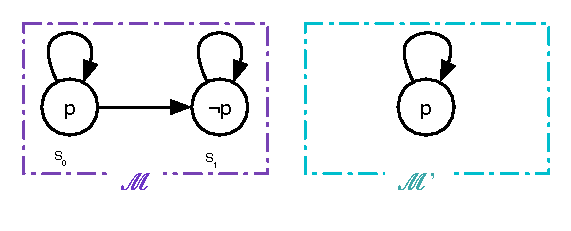
\includegraphics[width=1\textwidth]{Figures/State Diagram AGEFp}
    \label{figure:State_Diagram_AGEFp}
\end{figure}

% -- Bibliography -------------------------------------------------------------

% -- Document Bibliography ----------------------------------------------------

\IfFileExists{References.bib}{
    % Set section format for bibliography
    \titleformat{\section}{\sffamily\bfseries}{}{0pt}{}[{\color{aqua}\hrule}]
    % Display bibliography
    \printbibliography
}{}

\end{document}
